\section{Full Battery and Confidence Intervals}
\label{app:battery}

Table~\ref{tab:fullbattery} gives every condition with Wilson $95\%$ intervals
($N = 400$). Base A1/A2/D1 are not in our committed data and are omitted rather than
estimated.

\begin{table}[h]
\centering
\footnotesize
\setlength{\tabcolsep}{3pt}
\begin{tabular}{@{}llcc@{}}
\toprule
 & surface & base & instruct \\
\midrule
C0 & \texttt{B * C =} & .838\,{\scriptsize[.80,.87]} & .848\,{\scriptsize[.81,.88]} \\
C1 & \texttt{( 0 + B ) * C =} & .508\,{\scriptsize[.46,.56]} & .265\,{\scriptsize[.22,.31]} \\
C2 & \texttt{( 0 + B * C ) =} & n/a & .678\,{\scriptsize[.63,.72]} \\
C3 & \texttt{( B ) * C =} & n/a & .755\,{\scriptsize[.71,.80]} \\
C4 & \texttt{( B * C ) =} & .890\,{\scriptsize[.86,.92]} & .908\,{\scriptsize[.88,.93]} \\
C5 & \texttt{0 + B * C =} & n/a & .542\,{\scriptsize[.49,.59]} \\
C6 & \texttt{( 0 + B ) =} & 1.00\,{\scriptsize[.99,1.0]} & 1.00\,{\scriptsize[.99,1.0]} \\
C7 & \texttt{(0+B)*C=} & .018\,{\scriptsize[.01,.04]} & .190\,{\scriptsize[.16,.23]} \\
C8 & \texttt{(B*C)=} & .765\,{\scriptsize[.72,.80]} & .785\,{\scriptsize[.74,.82]} \\
A1 & \texttt{( 0 + B ) + C =} & n/a & .995\,{\scriptsize[.98,1.0]} \\
A2 & \texttt{0 + ( B + C ) =} & n/a & .928\,{\scriptsize[.90,.95]} \\
D1 & \texttt{(( 0 + B )) * C =} & n/a & .038\,{\scriptsize[.02,.06]} \\
\bottomrule
\end{tabular}
\caption{Full battery, exact-match accuracy with Wilson $95\%$ CIs. Note C5: relying on bare
operator precedence (\texttt{0 + B * C =}, $0.542$) beats the parenthesized additive identity
(C1, $0.265$), so the parenthesization actively hurts (instruct).}
\label{tab:fullbattery}
\end{table}

\paragraph{Magnitude control.} Within matched $|B\!\cdot\!C|$ bins (instruct), C1 vs C4:
$[440,813)$ .53/.96 ($n{=}79$); $[813,1185)$ .28/.94 (126); $[1185,1558)$ .16/.89 (104);
$[1558,1930)$ .19/.89 (64); $[1930,2303)$ .00/.70 (27). Every paired difference has a
positive bootstrap CI.

\section{Wrapper Blind-Spot Map}
\label{app:wrapper}
\begin{figure}[h]
\centering
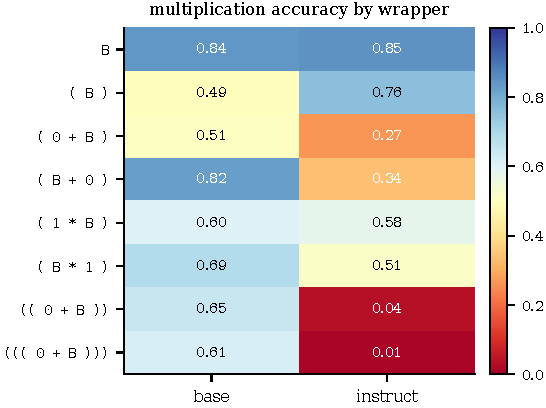
\includegraphics[width=0.82\columnwidth]{figs/figA_wrapper.pdf}
\caption{Multiplication accuracy by wrapper. Position-dependence is a base-model effect
(left-placed $(\,0{+}B\,)$ collapses, right-placed $(\,B{+}0\,)$ barely moves; instruct degrades
on both placements), and instruction tuning is not uniformly worse (plain parentheses).}
\label{fig:wrapper}
\end{figure}

\section{By-Layer Decodability}
\label{app:decode}
\begin{figure}[h]
\centering
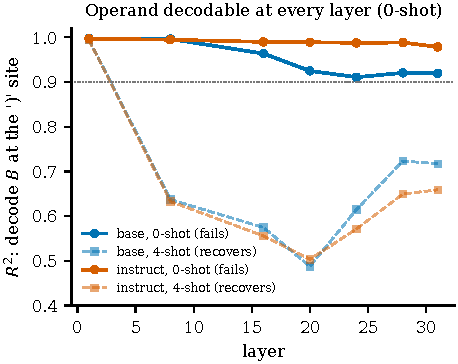
\includegraphics[width=0.82\columnwidth]{figs/figA_decode.pdf}
\caption{Operand $B$ decodes at every layer in the failing zero-shot regime (solid). The
few-shot curves (dashed) drop mid-network; shown for completeness only, and we draw no
mechanistic conclusion from the few-shot decodability.}
\label{fig:decode}
\end{figure}

\section{Steering Nulls}
\label{app:steering}
\begin{figure}[h]
\centering
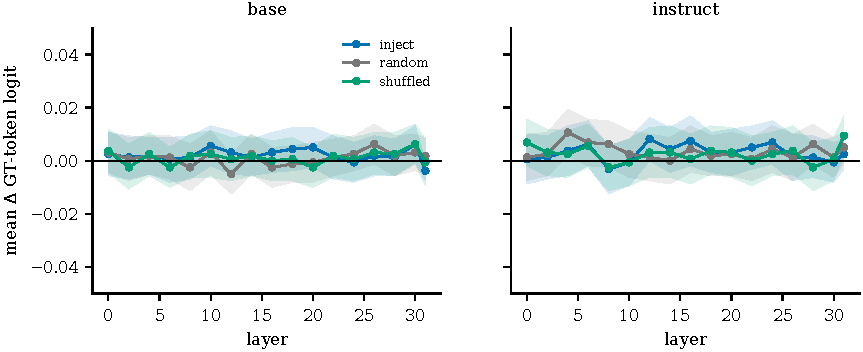
\includegraphics[width=\columnwidth]{figs/figA_steering.pdf}
\caption{Probe-direction steering at ``$=$'' is inert at every layer for inject, random,
and shuffled targets (mean $\Delta$ ground-truth-token logit, $95\%$ CIs through zero).
This first-token metric is a null; the discriminative full-product nulls are the dose-response
(\S\ref{sec:dormant}) and Figure~\ref{fig:evidence}b.}
\label{fig:steernull}
\end{figure}

\section{Cross-Model Battery}
\label{app:crossmodel}
Matched bare format, in scope if C4 and C6 $\geq 0.80$: Llama-3.1-8B base C1 $.508$ /
instruct $.265$; Gemma-2-9b-it $.043$ (C4 $.99$); Llama-3.2-3B $.358$ (C4 $.88$). Out of
scope (parts fail): Qwen2.5-7B (C4 $.00$), Mistral-7B (C4 $.62$), Llama-3.2-1B (C4 $.31$).
Chat format: Gemma-2-9b-it composes (C1 $.95$, C4 $.99$) but Llama-3.1-8B chat falls out of
scope (C4 $.70$); the composing and failing models are never in the same format.

\section{Proof of Proposition~\ref{prop:headroom}}
\label{app:proof}
The cross-validated coefficient of determination we report is $R^2 = 1 - \mathrm{SS_{res}}/\mathrm{SS_{tot}}$
with $\mathrm{SS_{res}} \ge 0$, so $R^2_{\mathrm{real}} \le 1$. The baseline probe is a restriction
of the same probe class to features $F$, hence $R^2_{F}$ is well defined on the same folds. Then
$\mathrm{gap} = R^2_{\mathrm{real}} - R^2_{F} \le 1 - R^2_{F}$, the headroom. Thus if the baseline
already explains the target on $D$ ($R^2_F \to 1$), the gap is forced to $0$ regardless of whether
the target is separately represented; the test is informative only in proportion to the headroom,
which must therefore be reported. At $[20,49]$ headroom $= 1 - 0.968 = 0.032$ (near-vacuous); at
$[2,99]$ headroom $= 1 - 0.865 = 0.135$, inside which the observed gap $0.060$--$0.068$ (CI excludes
$0$) lies. $\qed$

\section{A decodability-audit protocol}
\label{app:audit}
The claim ``value $v$ is computed at site $s$'' from a decodable probe should clear three checks.
(1) \textbf{Selectivity with headroom.} Report a gap over a stated baseline feature class and the
headroom $1 - R^2_F$ (Prop.~\ref{prop:headroom}); a gap in a headroom-less regime is uninformative.
(2) \textbf{A causal test on a discriminative metric with a same-axis reference that moves.} Steer
the decodable direction and score a metric that distinguishes the target from the status quo (here
a full-product log-probability, not a shared first token), and show the \emph{same} axis moves a
reference where the value is used. (3) \textbf{A positive control at a site that moves the answer},
so a null is a dead direction, not a dead instrument. Our answer-site subspace passes (1)'s form
but fails (2) and (3) at ``$=$''.

\section{Verbatim prompt strings}
\label{app:prompts}
Bare-continuation format (\texttt{prepend\_bos=True}), shown for $B{=}23, C{=}47$; spacing is exact.
\begin{quote}\ttfamily\small
C0: 23 * 47 =\\
C1: ( 0 + 23 ) * 47 =\\
C2: ( 0 + 23 * 47 ) =\\
C3: ( 23 ) * 47 =\\
C4: ( 23 * 47 ) =\\
C5: 0 + 23 * 47 =\\
C6: ( 0 + 23 ) =\\
C7: (0+23)*47=\\
C8: (23*47)=\\
A1: ( 0 + 23 ) + 47 =\\
A2: 0 + ( 23 + 47 ) =\\
D1: (( 0 + 23 )) * 47 =
\end{quote}
The few-shot C1 template prepends $k$ solved C1 lines (distinct operands, correct answers), newline
separated, then the target C1 line; e.g.\ \texttt{( 0 + 20 ) * 21 = 420$\backslash$n( 0 + 23 ) * 47 =}.

\section{The answer site is bypassed}
\label{app:emit_true}
After the full-residual swap at the C4 ``$=$'' site, the model emits neither the donor product
(emit-$P' = 0$ at every layer) nor a corrupted output: it emits its \emph{own} correct answer at
$0.90$--$0.95$ across L19--L31 (Table~\ref{tab:emit}). The site is demonstrably read past.

\begin{table}[h]
\centering
\footnotesize
\setlength{\tabcolsep}{4pt}
\begin{tabular}{@{}rcccc@{}}
\toprule
 & \multicolumn{2}{c}{base} & \multicolumn{2}{c}{instruct} \\
layer & logp$\Delta$ & emit-true & logp$\Delta$ & emit-true \\
\midrule
19 & $+0.59$ & 0.90 & $+0.12$ & 0.95 \\
23 & $+0.66$ & 0.92 & $+0.15$ & 0.92 \\
27 & $+0.53$ & 0.92 & $+0.13$ & 0.93 \\
31 & $+0.00$ & 0.92 & $+0.00$ & 0.92 \\
\bottomrule
\end{tabular}
\caption{Full-residual swap at C4 ``$=$'': emit-$P' = 0$ at every layer (omitted); the model keeps
emitting its own correct answer. \texttt{causal\_steering\_lateswap\_*.json}.}
\label{tab:emit}
\end{table}

\section{Baseline scope and reproducibility}
\label{app:repro}
\textbf{Baseline scope.} The linear-$(B,C)$ baseline's span excludes $B^2$, $C^2$, and
$B\!\cdot\!C$, so the band-$[2,99]$ gap upper-bounds operand-\emph{nonlinear} structure and is
consistent with, but does not identify, a product component; a quadratic-feature baseline is the
decisive test. \textbf{Reproducibility.} All results use greedy decoding, integer parsing
(parse-fail counts as incorrect), $N = 400$ operand pairs, seed $0$, \texttt{prepend\_bos=True},
\texttt{pairs\_sha=db4da1}, on Llama-3.1-8B base (\texttt{meta-llama/Llama-3.1-8B}) and instruct
(rev \texttt{0e9e39f}) in bf16 on an NVIDIA A100; TransformerLens 3.5.0, torch 2.11, transformers
5.12.
